\chapter{Mission 1: Your First Blocks}
\label{ch:kids1}

\begin{prgteacher}
Part~IV is written for children from about seven years old, working with a
teacher, parent, or older student. The sentences are short on purpose, and the
child is addressed directly. Read the chapter aloud with younger pupils; let
older ones read it themselves. Everything an adult needs, from installation to
lesson plans and assessment, is in Chapter~\ref{ch:kitteach}. No hardware is
required: the whole track runs in a web browser.
\end{prgteacher}

Hello, maker! In this part of the book \textbf{you} are going to build video
games. Real ones. You will not type long lines of strange words. You will snap
coloured \emph{blocks} together, like building bricks, and the computer will do
what your blocks say.

\section{What is a program?}

A computer is very fast, but it is not clever. It cannot guess what you want. It
only follows instructions, one after another, exactly as they are written.

A list of instructions for a computer is called a \textbf{program}. A person who
writes programs is called a \textbf{programmer}. Today, that is you.

\begin{prgtry}
Play \emph{Robot} with a friend. You are the programmer; your friend is the
robot. The robot may only do what you say: ``one step forward'', ``turn left'',
``pick up the pencil''. Can you get your robot from the door to the window? What
happens if you forget one instruction?
\end{prgtry}

\section{Meet the Construction Kit}

The tool you will use is called the \textbf{PRG32 Construction Kit}
\citep{prg32kit}. It opens in a web browser, like a web page. Your teacher will
give you the address.

\begin{center}
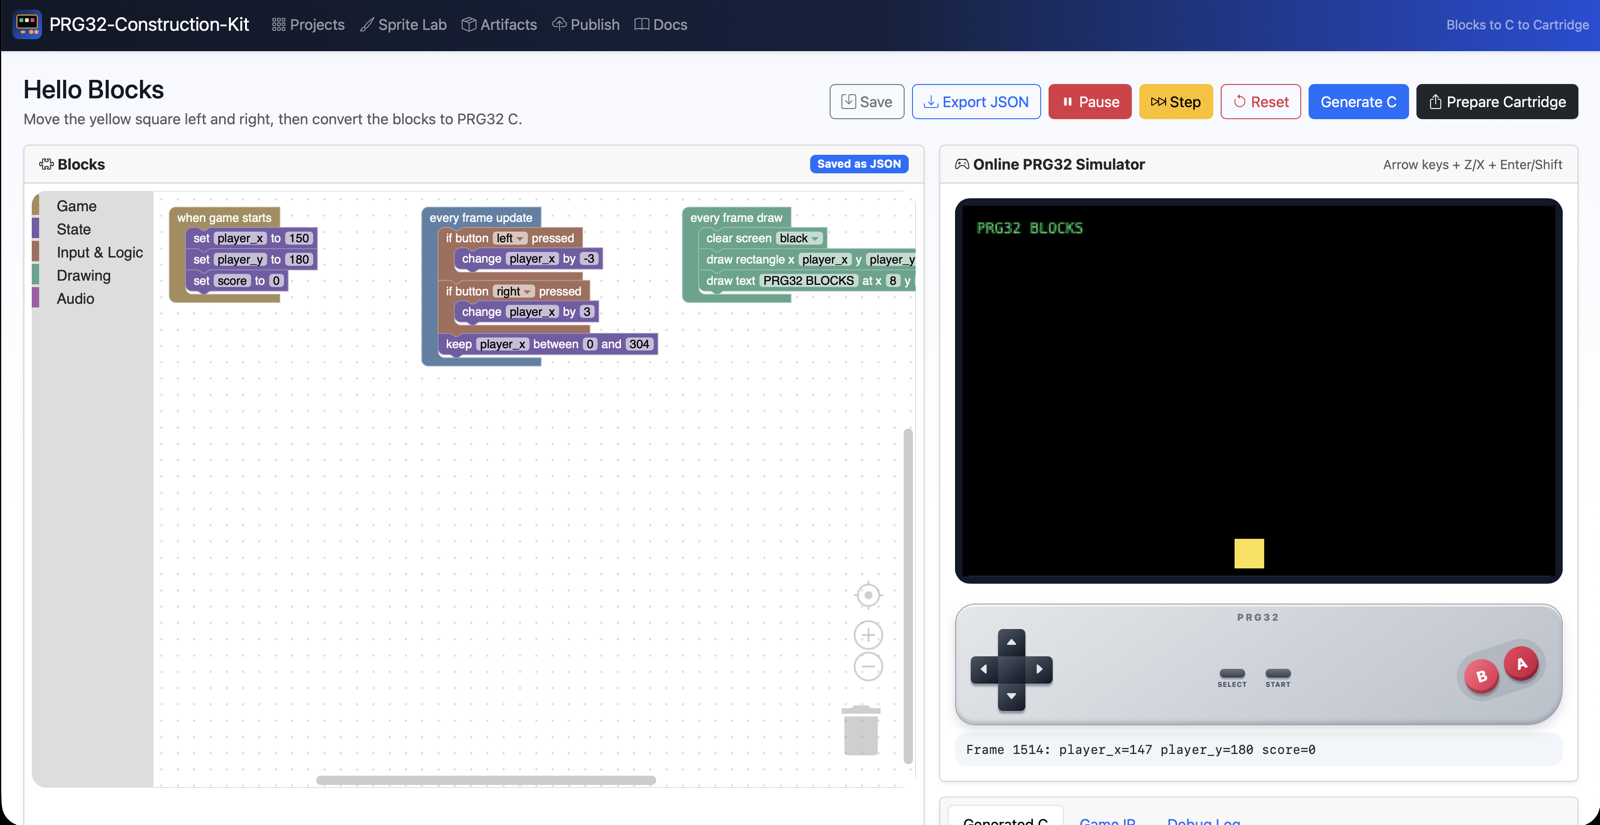
\includegraphics[width=\linewidth]{figures/construction-kit-editor.png}
\captionof{figure}{The Construction Kit. On the left are the blocks. On the
right is the game screen, with a game pad under it \citep{prg32kit}.}
\label{fig:kiteditor}
\end{center}

Look for these four places on the screen:

\begin{itemize}
  \item the \textbf{toolbox}, where the blocks live, sorted by colour;
  \item the \textbf{workspace}, the big empty area where you build;
  \item the \textbf{game screen}, where your game appears;
  \item the \textbf{buttons} at the top: \kbtn{Save}, \kbtn{Play}, \kbtn{Step},
        and \kbtn{Reset}.
\end{itemize}

\begin{prgmission}[Mission 1, step 1: a new project]
\begin{enumerate}
  \item Click \kbtn{New Project}.
  \item Type the title \textbf{First Square}.
  \item Click \kbtn{Create}.
\end{enumerate}
\end{prgmission}

\section{The screen is a grid}

The game screen is made of tiny squares called \textbf{pixels}. There are 320
pixels from left to right and 200 pixels from top to bottom.

To tell the computer \emph{where} to draw, you give it two numbers:

\begin{itemize}
  \item \textbf{x} says how far to the \emph{right};
  \item \textbf{y} says how far \emph{down}.
\end{itemize}

\begin{center}
\begin{tikzpicture}[font=\sffamily\small,scale=0.9]
  \draw[draw=prgink!60,fill=prgink!6,thick] (0,0) rectangle (8,5);
  \fill[prgred] (0,5) circle (2pt) node[above right,text=prgred]{x = 0, y = 0};
  \draw[-{Stealth[length=2.5mm]},thick,prgaccent] (0.4,4.6) -- (3.2,4.6)
    node[right]{x gets bigger};
  \draw[-{Stealth[length=2.5mm]},thick,prgviolet] (0.4,4.6) -- (0.4,2.2)
    node[below right]{y gets bigger};
  \fill[prgamber] (5.3,2.3) rectangle (5.7,2.7);
  \node[below] at (5.5,2.25){x = 152, y = 92};
  \node[anchor=south east] at (8,0.05){x = 319, y = 199};
\end{tikzpicture}
\captionof{figure}{The game screen. The corner at the top left is the
starting point. Going right makes x bigger. Going \emph{down} makes y bigger.}
\label{fig:kidgrid}
\end{center}

\begin{prgwarn}
On a game screen, a \emph{bigger} y is \emph{lower} down. That feels upside
down at first. If something goes down when you wanted up, check your y.
\end{prgwarn}

\section{Three big blocks}

Every game you make has three big yellow blocks. They are in the \textbf{Game}
drawer of the toolbox.

\kgame{when game starts}
\kgame{every frame update}
\kgame{every frame draw}

\begin{itemize}
  \item \textbf{when game starts} runs \emph{one time}, at the beginning. Here
        you get things ready.
  \item \textbf{every frame update} runs again and again, many times each
        second. Here you \emph{change} things.
  \item \textbf{every frame draw} also runs again and again. Here you
        \emph{paint} the picture.
\end{itemize}

A \textbf{frame} is one picture. A cartoon is many pictures shown very quickly,
one after another. A game is the same: get ready once, then change, paint,
change, paint, change, paint\dots

\begin{prgconcept}
A game is a loop. First it gets ready. Then it repeats two jobs forever:
\emph{update} (change the numbers) and \emph{draw} (paint the picture).
\end{prgconcept}

\section{Boxes with names: variables}

A game must remember things: where the player is, how many points you have. It
keeps each thing in a \textbf{variable}. A variable is a box with a name on it
and one number inside.

\begin{center}
\begin{tikzpicture}[font=\sffamily\small]
  \foreach \x/\name/\val in {0/player\_x/152,3.4/player\_y/92}{
    \draw[thick,draw=prgviolet,fill=prgviolet!10,rounded corners=2pt] (\x,0) rectangle ++(2.6,1.4);
    \node[font=\sffamily\bfseries\Large] at (\x+1.3,0.7){\val};
    \node[above,text=prgviolet] at (\x+1.3,1.4){\name};
  }
\end{tikzpicture}
\captionof{figure}{Two variables. Each is a named box with a number inside.}
\end{center}

The purple block \textbf{set} puts a number in a box.

\begin{prgmission}[Mission 1, step 2: get ready]
Drag \textbf{when game starts} into the workspace. Open the purple
\textbf{State} drawer and snap two \textbf{set} blocks inside it. Change the
words and numbers so it looks like this:

\kgame{when game starts}
\kstate[6mm]{set player\_x to 152}
\kstate[6mm]{set player\_y to 92}
\end{prgmission}

\section{Paint the picture}

Now tell the computer what to paint. The green-blue blocks in the
\textbf{Drawing} drawer do that.

\begin{prgmission}[Mission 1, step 3: draw]
Drag \textbf{every frame draw} into the workspace and fill it like this:

\kgame{every frame draw}
\kdraw[6mm]{clear screen BLACK}
\kdraw[6mm]{draw rectangle x player\_x y player\_y w 16 h 16 color YELLOW}
\kdraw[6mm]{draw text HELLO PRG32 at x 8 y 8 fg GREEN bg BLACK}

In the rectangle block, \textbf{w} is how wide and \textbf{h} is how high.
\end{prgmission}

Why \textbf{clear screen} first? Because the computer paints on top of the old
picture. If you do not clean the screen, the old drawings stay.

\begin{prgmission}[Mission 1, step 4: play!]
Click \kbtn{Save}. Then click \kbtn{Play}.

You should see a yellow square in the middle of a black screen, and green words
at the top. You made that!
\end{prgmission}

\section{Change one thing}

Real programmers learn by changing \emph{one} thing and watching what happens.
Try these. After each change, press \kbtn{Reset} and \kbtn{Play}.

\begin{prgtry}
\begin{enumerate}
  \item Change \textbf{player\_x} to 0. Where did the square go?
  \item Change \textbf{player\_x} to 304. Where is it now?
  \item Change \textbf{player\_y} to 184. Is the square higher or lower?
  \item Make the square 64 wide and 8 high. What shape is it?
  \item Change the colour. Change the words.
  \item Add a second rectangle with a different colour. Can you draw a house?
\end{enumerate}
\end{prgtry}

\begin{prgwarn}
The order of blocks matters. Put \textbf{clear screen} \emph{under} your
rectangle and press Play. The square is gone! The computer painted the square,
then painted black over it.
\end{prgwarn}

\section{When something goes wrong}

Mistakes in a program are called \textbf{bugs}. Everybody makes them. Finding
and fixing a bug is called \textbf{debugging}, and it is part of the fun.

\begin{itemize}
  \item \textbf{Nothing on the screen?} Did you press \kbtn{Play}? Is your
        rectangle inside \emph{every frame draw}?
  \item \textbf{Square in the wrong place?} Read your x and y numbers aloud.
  \item \textbf{A block will not snap in?} Blocks only fit inside one of the
        three big yellow blocks.
\end{itemize}

\begin{prgcheck}
You finished Mission~1 if you can:
\begin{itemize}
  \item say what a program is;
  \item point to the top-left corner and say its x and y;
  \item name the three big blocks and say when each one runs;
  \item say what a variable is;
  \item move your square by changing a number.
\end{itemize}
\end{prgcheck}

\begin{prggrownup}
The finished project is in the book's repository as
\fname{examples/blocks\_first\_steps/first\_square.blocks.json}; use
\kbtn{Import JSON} on the Kit's home page to load it. The ``Robot'' game is an
unplugged activity in the tradition of \citet{bell2009}; it is worth ten minutes
before any screen is switched on.
\end{prggrownup}
